\subsubsection{Multilayer Perceptron}
\label{sec:mlp-multilayer-perceptron}
A multilayer perceptron consists of multiple perceptrons divided in layers and solves complex tasks.
It is an universal approximator for every function\cite{Cybenko1989} regardless of the activation functions used\cite{Hornik1991}.
Because of the multiple layers and the non-linear activation functions non-linearity is introduced into the network.
Thus, it can distinguish data that is not linearly separable as most real world data is.

There are at least three layers.
Each layer contains several perceptrons that are not connected to each other.
However, every perceptron is connected to every perceptron of its subsequent layer.
This type of connection is called fully-connected network.
Because the data flow within the network is only in one direction and does not contain circles, the architecture is called feedforward neural network.
A visualization of this is shown in \figref{fig:multilayer-perceptron}.
Although the weights are not displayed for clarity, they still exist and follow the same principle as with a single perceptron.
\begin{figure}
	\centering
	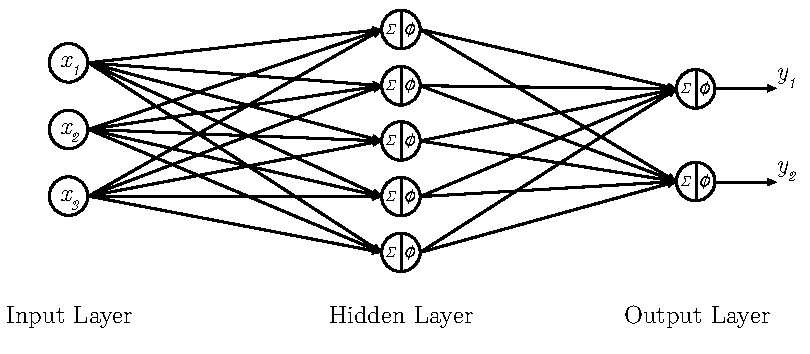
\includegraphics{images/multilayer-perceptron}
	\caption{Multilayer Perceptron}
	\label{fig:multilayer-perceptron}
\end{figure}
Like the single perceptrons every node in the networks still holds a single numerical value.
In this kind of network architecture perceptrons are often referred to as nodes.

The input layer serves as an interface for the data.
It does not perform any calculations and just passes the data to the next layer.
The number of nodes in this layer depends on the data and how it can be divided.
If the real world data is an image, for example, the number of nodes should be equal to the number of pixels, so that every node can hold the intensity value of one pixel.

The output layer is responsible for transferring the network data to the outside so that it can be interpreted and worked with.
The number of nodes in this layer depends on the expected results.
If kinds of animals need to be detected in an image, every output node would represent a single kind or category, respectively.
Let's say there are three kinds of animals possible, then there need to be three output nodes.
In theory the node representing the correct kind of animal holds a one and every other a zero, if the values are squashed within this range.

Every layer between the input and the output layer is a hidden layer.
They have no direct connection to the outside, neither to the input nor the output, hence, their name.
Their task is to transfer the input information to the output by performing calculations.
With at least one hidden layer every continuous function can be approximated.

Let's take again an image as an example.
The task is to classify a handwritten digit from the MNIST dataset\cite{Lecun98}
\begin{figure}
	\centering
	\includegraphics{images/mnist-digit}
	\caption[Handwritten Digit from the MNIST Digit Dataset]{Handwritten Digit from the MNIST Digit Dataset. Represented as a $28 \times 28$ pixel matrix. Each cell represents a pixel.}
	\label{fig:mnist-digit}
\end{figure}
The digit can be seen in \figref{fig:mnist-digit}.
Each grid cell represents a pixel.
Because every pixel should have an associated node in the input layer of the network, this real world data is transferred into the network by flattening the intensity values of the image matrix to a vector.
Therefore, the vector contains $28 \cdot 28 = 784$ elements which equals the number of input nodes.
If the correct weights and biases of the network are found, it knows that if in another image more or less the same pixels or nodes, respectively, have high intensities, the same number is written.
The downside of the flattening is, that every relation of pixels like position is lost, which means a loss in overall information.
The consequence of this is, that if a digit is not centered and, for example, takes only half the space of the image, it cannot be classified, because the network has never seen something similar to these input values.
